\chapter{Routing e Trasporto nelle Reti Wireless}
Finora abbiamo guardato al livello fisico e al MAC di una singola cella. In questo capitolo saliamo ai livelli rete e trasporto in scenari wireless multi-hop, dove i pacchetti devono attraversare più nodi intermedi. Il contesto di riferimento sono le \textbf{reti ad hoc mobili (MANET)}, in cui dispositivi wireless mobili formano una rete senza infrastruttura preesistente.

\section{Reti Ad Hoc Mobili (MANET)}
\dfn{MANET (Mobile Ad Hoc Network)}{
    Una rete formata da host wireless eventualmente mobili, \emph{senza} (necessariamente) un'infrastruttura preesistente. Le rotte tra i nodi possono attraversare più hop, e la mobilità causa continui cambiamenti di topologia (rottura e creazione di link).
}

\begin{center}
    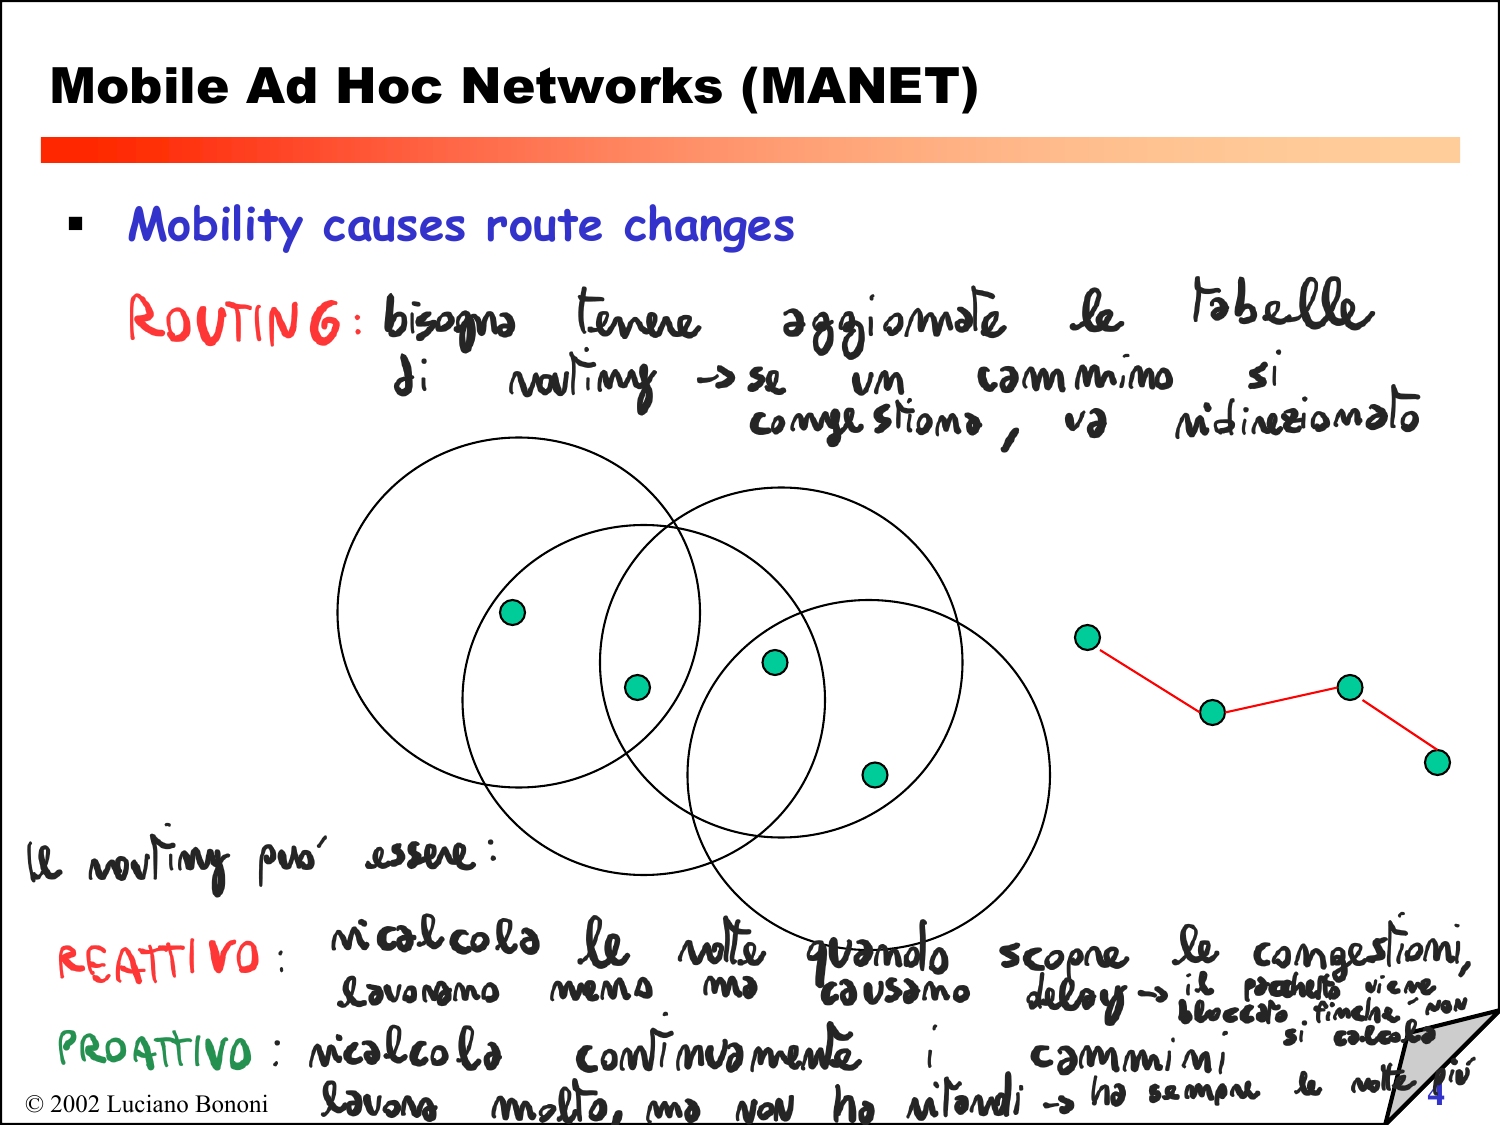
\includegraphics[width=9cm]{img/manet.png}
\end{center}

\subsection{Perché il routing in MANET è diverso?}
\begin{itemize}
    \item \textbf{Mobilità degli host}: i guasti/ripristini dei link dovuti al movimento hanno caratteristiche diverse da quelli di altre cause, e il loro tasso può essere elevato (nodi che si muovono velocemente).
    \item \textbf{Nuovi criteri di prestazione}: oltre alla lunghezza del cammino contano la \textbf{stabilità della rotta} rispetto alla mobilità e il \textbf{consumo energetico} (batterie).
    \item Nessun protocollo funziona bene in tutti gli ambienti: la scelta dipende dai pattern di traffico e di mobilità.
\end{itemize}

\subsection{Classificazione dei protocolli di routing}
\begin{itemize}
    \item \textbf{Proattivi}: determinano le rotte \emph{indipendentemente} dal traffico, mantenendole sempre aggiornate. Sono di questo tipo i tradizionali protocolli \textit{link-state} e \textit{distance-vector}.
    \item \textbf{Reattivi (on-demand)}: mantengono una rotta \emph{solo se serve}, scoprendola al momento del bisogno.
    \item \textbf{Ibridi}: combinano i due approcci.
\end{itemize}

\dfn{Trade-off proattivo vs reattivo}{
    I protocolli \textbf{proattivi} hanno minore \emph{latenza} di scoperta (le rotte sono già pronte), ma maggiore \emph{overhead} per l'aggiornamento continuo. I protocolli \textbf{reattivi} hanno minore overhead (cercano solo le rotte necessarie), ma maggiore latenza (una rotta da X a Y si trova solo quando X deve inviare a Y). Quale offra il compromesso migliore dipende dai pattern di traffico e mobilità.
}

\section{Flooding per la consegna dei dati}
La strategia più semplice per recapitare un pacchetto senza conoscere una rotta è il \textbf{flooding}.

\dfn{Flooding}{
    Il mittente S invia il pacchetto in broadcast a tutti i vicini; ogni nodo che lo riceve per la prima volta lo ri-trasmette ai propri vicini. I \textbf{numeri di sequenza} evitano che un nodo inoltri due volte lo stesso pacchetto. La destinazione D, raggiunta se connessa a S, non inoltra il pacchetto.
}

\begin{center}
    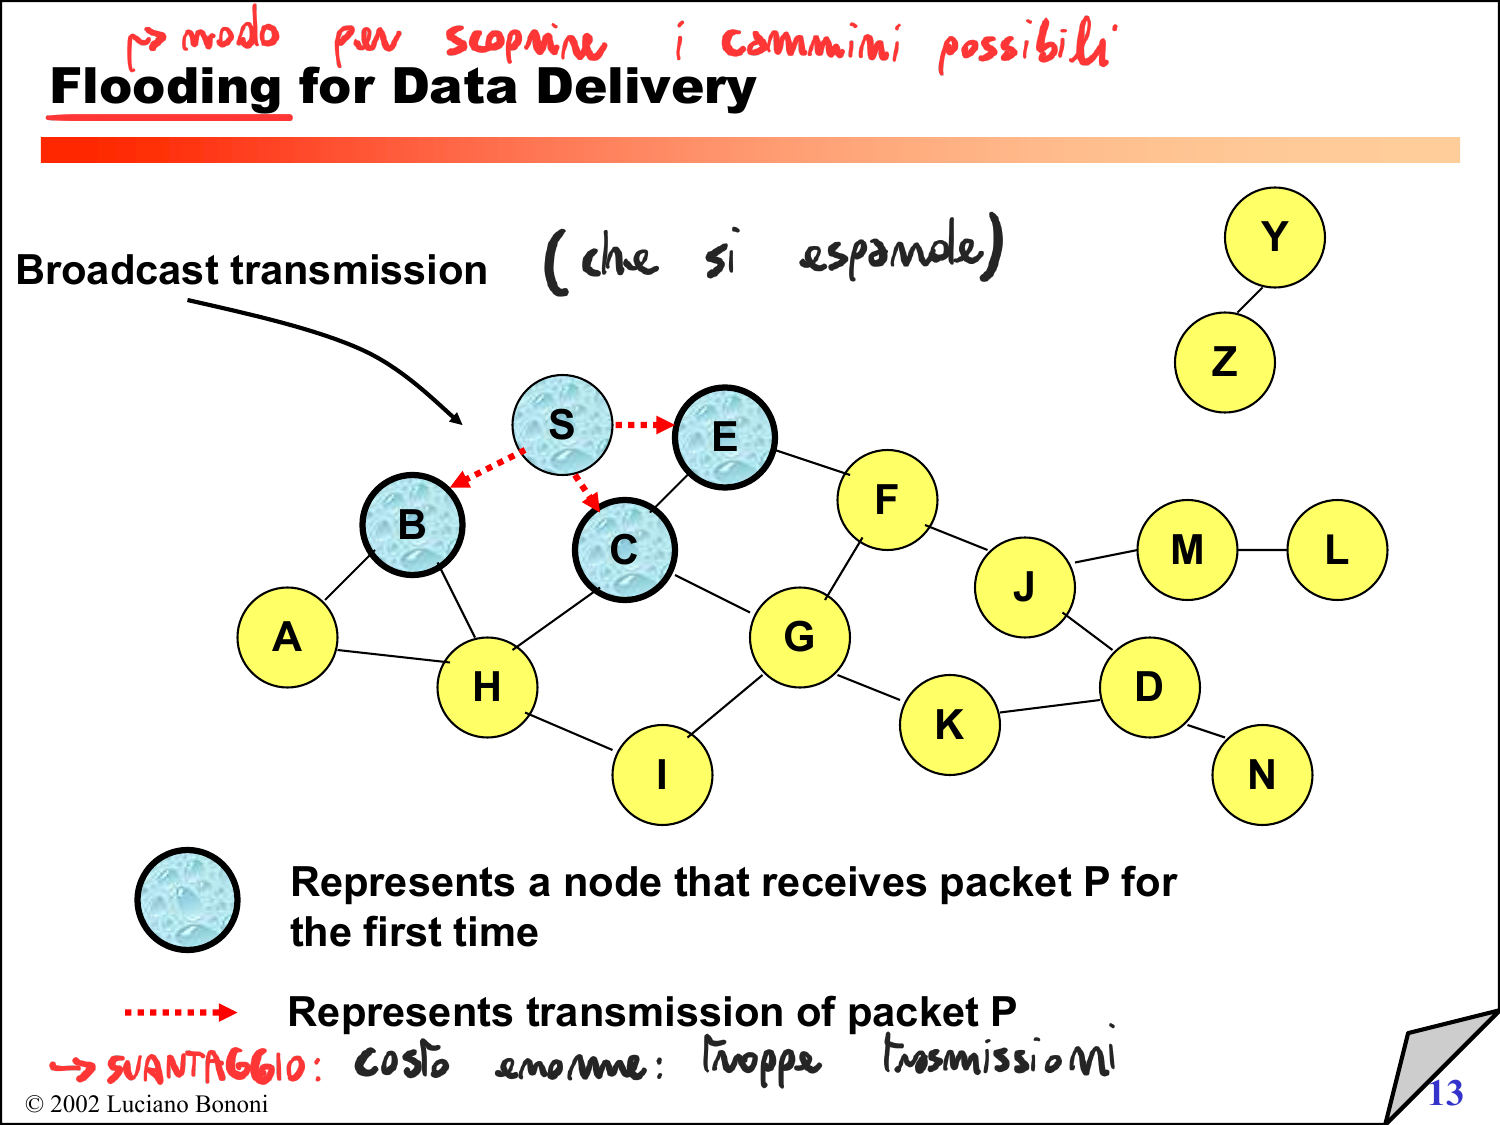
\includegraphics[width=9cm]{img/flooding.png}
\end{center}

\paragraph{Vantaggi.} Semplicità; può essere più efficiente di altri protocolli quando il traffico è così sporadico che l'overhead di una scoperta esplicita della rotta non sarebbe ammortizzato; potenziale maggiore affidabilità (il pacchetto può arrivare a D su più cammini).

\paragraph{Svantaggi.} Overhead potenzialmente altissimo (il pacchetto raggiunge anche nodi che non ne hanno bisogno); affidabilità potenzialmente bassa, perché il broadcast in 802.11 è \emph{non affidabile} (nessun ACK): due nodi nascosti che inoltrano contemporaneamente verso D possono collidere, e il pacchetto può non arrivare affatto.

\section{Dynamic Source Routing (DSR)}
Il DSR è un protocollo \textbf{reattivo} basato sul \textit{source routing}: la rotta completa è inclusa nell'header del pacchetto.

\subsection{Route Discovery}
Quando S vuole inviare a D ma non conosce una rotta, avvia una \textbf{route discovery}:
\begin{enumerate}
    \item S inonda la rete con un \textbf{Route Request (RREQ)}.
    \item Ogni nodo che inoltra l'RREQ \textbf{appende il proprio identificativo} alla lista nel pacchetto.
    \item Un nodo non inoltra due volte lo stesso RREQ.
\end{enumerate}

\begin{center}
    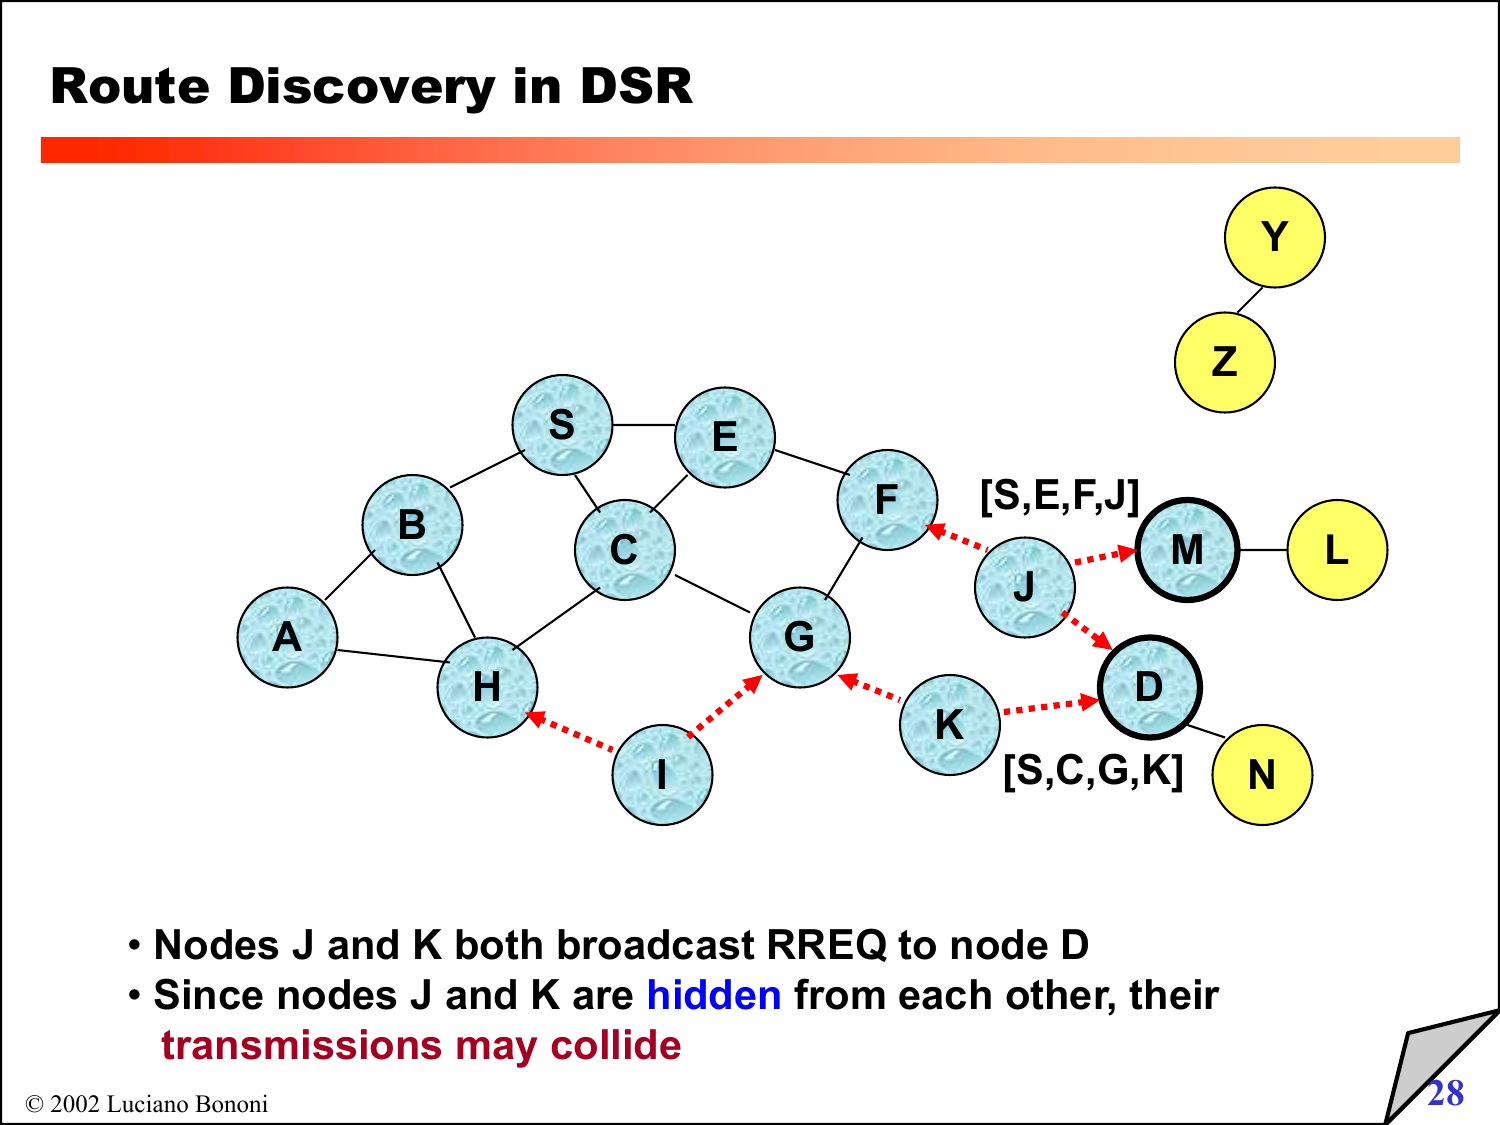
\includegraphics[width=9cm]{img/dsr_route_discovery.png}
\end{center}

\subsection{Route Reply}
Quando D riceve il \emph{primo} RREQ, invia un \textbf{Route Reply (RREP)} contenente la rotta accumulata da S a D.

\begin{center}
    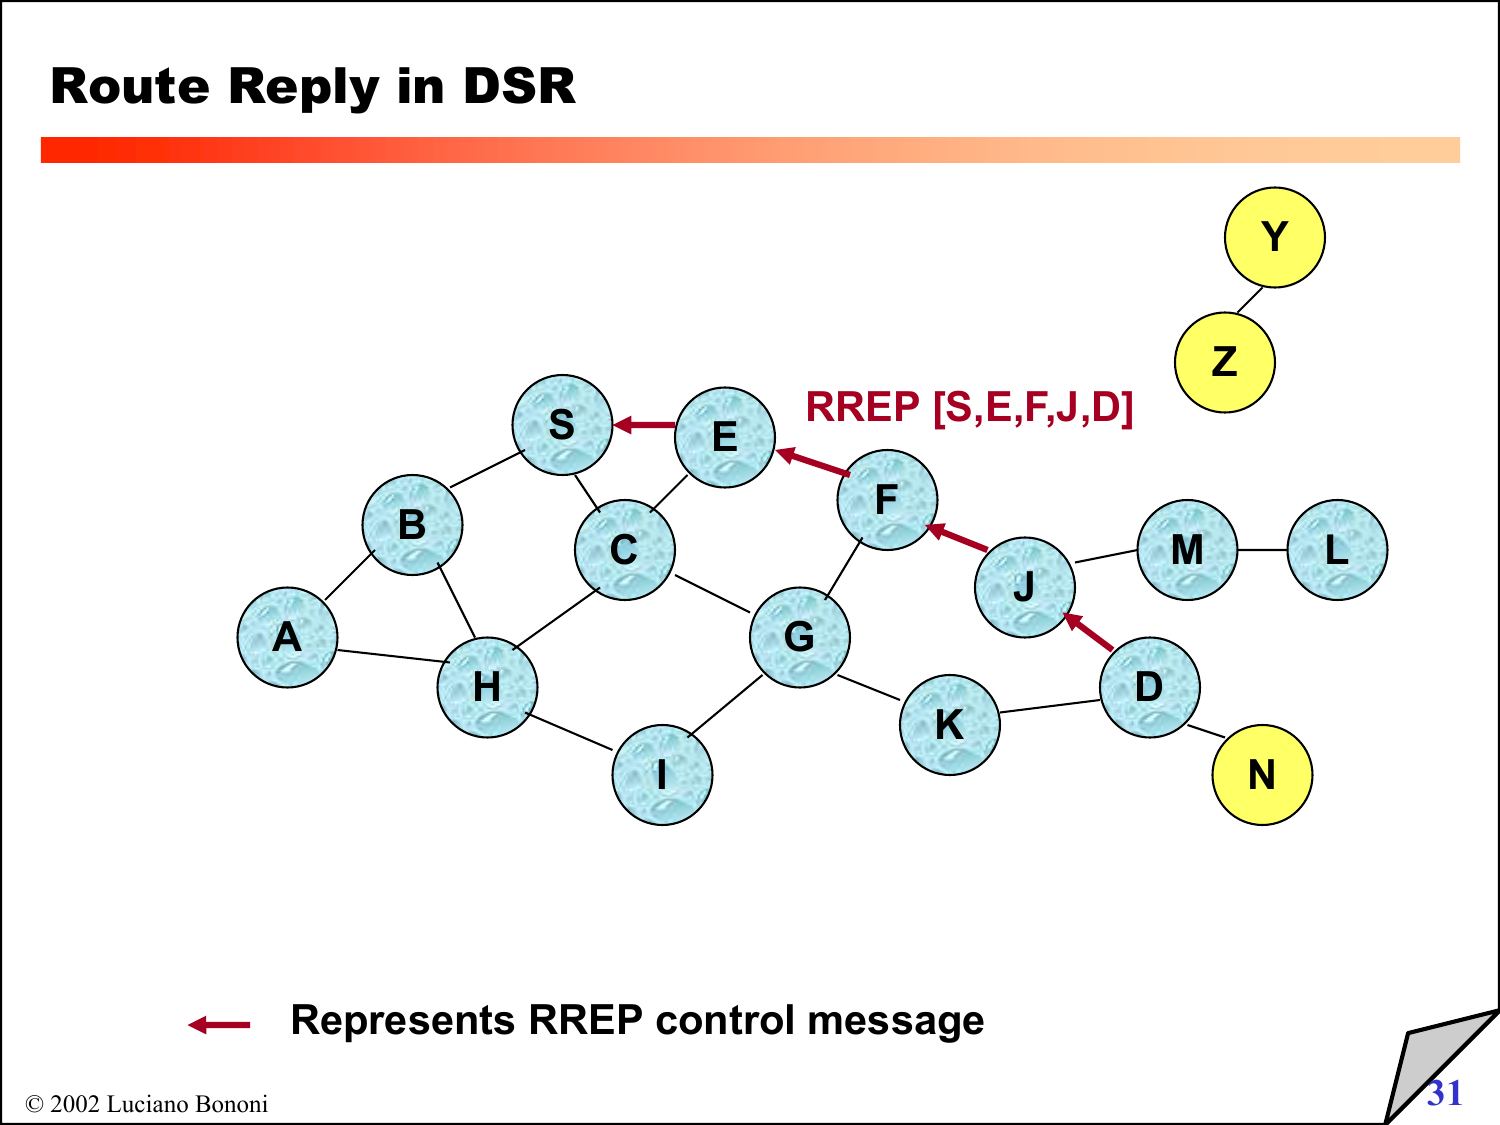
\includegraphics[width=9cm]{img/dsr_route_reply.png}
\end{center}

\nt{L'RREP può essere inviato semplicemente \textbf{invertendo} la rotta dell'RREQ solo se i link sono \emph{bidirezionali}. Se sono ammessi link unidirezionali (asimmetrici), D potrebbe dover avviare una propria route discovery verso S (con l'RREP in piggyback). Usando il MAC 802.11, che richiede ACK, i link sono comunque bidirezionali.}

S, ricevuto l'RREP, mette in cache la rotta e la include nell'header di ogni pacchetto dati (\emph{source routing}); i nodi intermedi inoltrano in base alla rotta scritta nel pacchetto.

\subsection{Route Caching}
Ottimizzazione fondamentale: ogni nodo \textbf{memorizza in cache} ogni rotta che apprende, comunque la apprenda.
\begin{itemize}
    \item Scoprendo $[S,E,F,J,D]$, S apprende anche la sotto-rotta $[S,E,F]$ verso F.
    \item Inoltrando un RREP o anche solo \emph{origliando} (overhearing) pacchetti dati, un nodo apprende rotte verso altre destinazioni.
    \item Un nodo che riceve un RREQ e \emph{conosce già} una rotta verso D può rispondere direttamente con un RREP, \textbf{velocizzando} la scoperta e \textbf{riducendo} la propagazione degli RREQ.
\end{itemize}

\dfn{Route Error (RERR)}{
    Quando un nodo non riesce a inoltrare un pacchetto su un link (es. J non raggiunge più D), invia un \textbf{RERR} al mittente lungo la rotta inversa. I nodi che lo sentono rimuovono il link rotto dalla propria cache.
}

\paragraph{Vantaggi.} Rotte mantenute solo tra nodi che comunicano; il caching riduce ulteriormente l'overhead; una singola discovery può fruttare più rotte (grazie ai nodi che rispondono dalla cache).

\paragraph{Svantaggi.}
\begin{itemize}
    \item L'header cresce con la lunghezza della rotta (source routing).
    \item Il flood di RREQ può raggiungere tutta la rete; servono ritardi casuali prima di inoltrare per evitare collisioni tra RREQ vicini.
    \item \textbf{Route Reply Storm}: se molti nodi rispondono dalla cache, aumenta la contesa. Si mitiga impedendo a un nodo di inviare l'RREP se sente un altro RREP con una rotta più corta.
    \item \textbf{Cache obsolete}: con la mobilità, rotte in cache diventano invalide; un nodo può rispondere con una rotta vecchia "inquinando" le cache altrui. Servono meccanismi di scadenza (timeout statici o adattivi basati sulla stabilità dei link).
\end{itemize}

\section{Riduzione del flooding: routing geografico}
Per limitare l'ambito del flood di route request si può sfruttare l'\textbf{informazione di posizione} (es. da GPS).

\subsection{Location-Aided Routing (LAR)}
\dfn{Expected Zone e Request Zone}{
    La \textbf{Expected Zone} è la regione in cui ci si aspetta si trovi la destinazione D, stimata dall'ultima posizione nota di D (al tempo $t_0$) e dalla sua velocità: un cerchio di raggio $r = (t_1 - t_0)\cdot v_{stima}$. La \textbf{Request Zone} è la regione che contiene la Expected Zone e il mittente S: solo i nodi \emph{dentro} la request zone inoltrano l'RREQ.
}

\begin{center}
    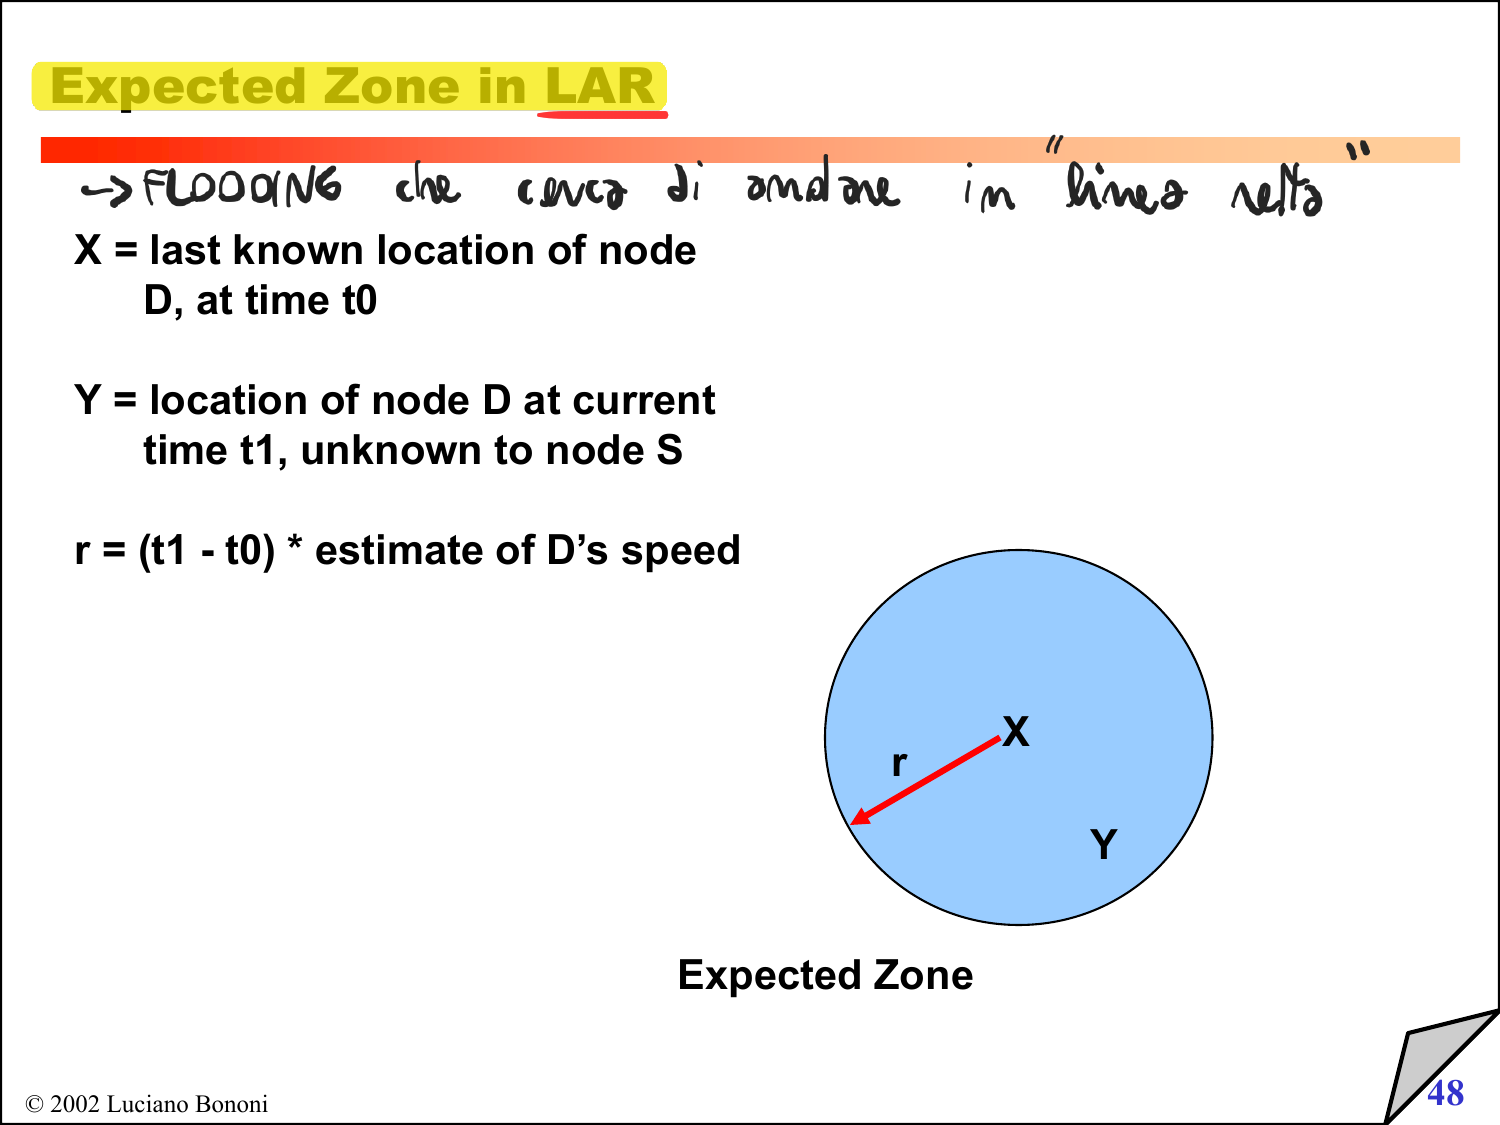
\includegraphics[width=7cm]{img/lar_expected_zone.png}
\end{center}

Se la discovery con request zone piccola fallisce, S ritenta (dopo un timeout) con una zona più ampia (al limite l'intera rete). \textbf{Vantaggi}: riduce l'ambito del flood e l'overhead. \textbf{Svantaggi}: i nodi devono conoscere la propria posizione fisica; non tiene conto di possibili ostacoli alla propagazione radio.

\subsection{Altri schemi geografici}
\begin{itemize}
    \item \textbf{DREAM} (Distance Routing Effect Algorithm for Mobility): inoltra i dati ai vicini contenuti in un "cono" diretto verso la expected zone della destinazione.
    \item \textbf{GEDIR} (Geographic Distance Routing): nota la posizione di D e dei propri vicini, ogni nodo inoltra il pacchetto al vicino \emph{più vicino} alla destinazione. Varianti con "guaranteed delivery" sanno aggirare gli ostacoli garantendo la consegna se un cammino esiste.
\end{itemize}

\section{Ad Hoc On-Demand Distance Vector (AODV)}
L'AODV migliora il DSR mantenendo \textbf{tabelle di routing} nei nodi, così che i pacchetti dati non debbano contenere l'intera rotta (header piccoli). Mantiene la caratteristica reattiva: rotte solo tra nodi che comunicano.

\dfn{Reverse path e Forward path}{
    Gli RREQ si propagano come nel DSR; quando un nodo ri-trasmette un RREQ, imposta un \textbf{reverse path} (puntatore verso il mittente). Quando D riceve l'RREQ risponde con un RREP che viaggia lungo il reverse path; al suo passaggio si impostano i \textbf{forward path} (voci di tabella verso la destinazione). AODV assume link \emph{simmetrici} (bidirezionali).
}

\begin{center}
    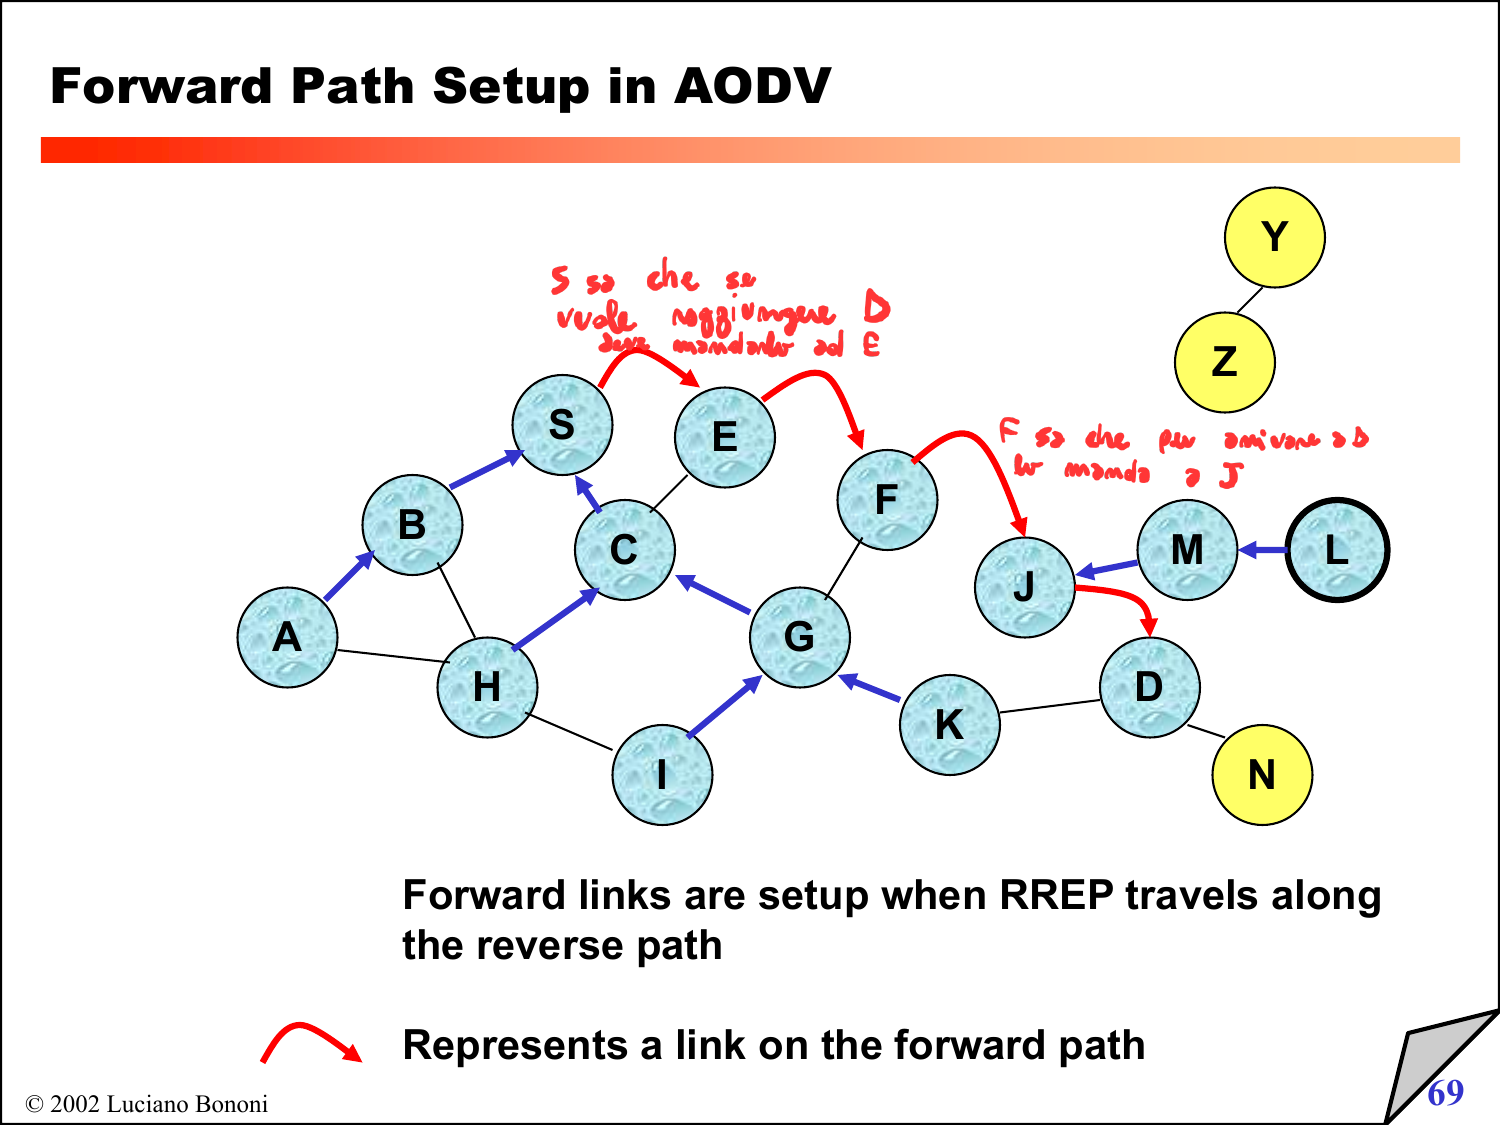
\includegraphics[width=9cm]{img/aodv_forward_path.png}
\end{center}

\dfn{Destination Sequence Number}{
    Numero di sequenza associato a ogni destinazione, usato per garantire la \emph{freschezza} delle rotte ed evitare loop. Un nodo intermedio può rispondere con un RREP solo se conosce una rotta con sequence number \emph{maggiore o uguale} a quello richiesto; una rotta più vecchia (numero più piccolo) non può essere usata per rispondere.
}

\paragraph{Timeout.} Una voce di reverse path scade dopo un intervallo (sufficiente a far tornare l'RREP). Una voce di forward path scade se non usata per un \texttt{active\_route\_timeout}: le rotte inutilizzate vengono cancellate anche se la topologia non è cambiata.

\nt{\textbf{DSR vs AODV}: DSR include la rotta nell'header (header grandi, ma può mantenere più rotte per destinazione e i nodi intermedi rispondono più spesso dalla cache); AODV usa tabelle (header piccoli, \emph{un solo} next-hop per destinazione, rotte che scadono se inutilizzate).}

\section{Protocolli proattivi: OLSR}
Tra i protocolli proattivi, il \textbf{link-state} classico fa sì che ogni nodo inondi periodicamente lo stato dei propri link. L'OLSR ottimizza questo flooding.

\dfn{OLSR e Multipoint Relays (MPR)}{
    In \textbf{OLSR} (Optimized Link State Routing) ogni nodo seleziona tra i suoi vicini un piccolo insieme di \textbf{multipoint relays (MPR)}: solo gli MPR ri-trasmettono le informazioni di stato, riducendo i broadcast ridondanti. Le rotte calcolate usano come nodi intermedi solo gli MPR.
}

\begin{center}
    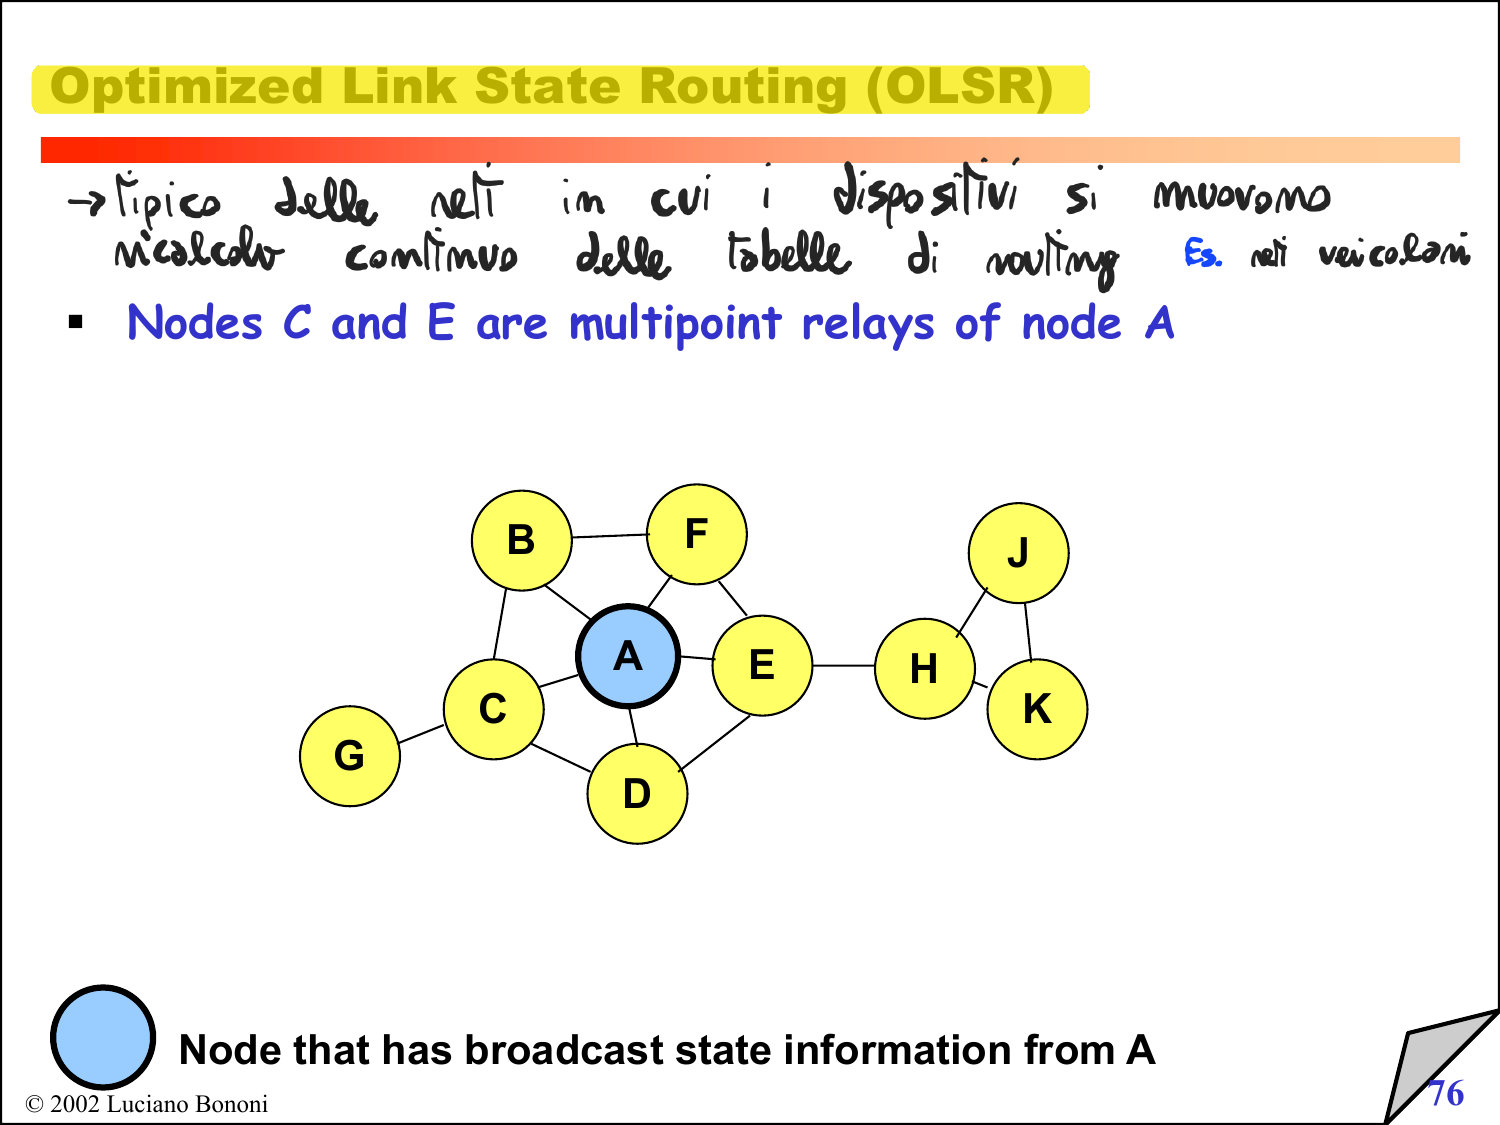
\includegraphics[width=8cm]{img/olsr_mpr.png}
\end{center}

\section{Mobile IP}
Quando un host mobile cambia rete IP, il suo indirizzo dovrebbe cambiare, interrompendo le connessioni in corso. \textbf{Mobile IP} risolve il problema mantenendo un indirizzo stabile.

\dfn{Home Agent e Foreign Agent}{
    L'\textbf{Home Agent (HA)} risiede nel router della rete "di casa" dell'host X e ne conosce sempre la posizione. Quando X si sposta in una rete estera, un \textbf{Foreign Agent (FA)} gli assegna un indirizzo temporaneo (care-of address) e informa l'HA. L'HA \textbf{incapsula (tunnel)} i pacchetti destinati a X e li inoltra al FA corrente, che li consegna a X.
}

\begin{center}
    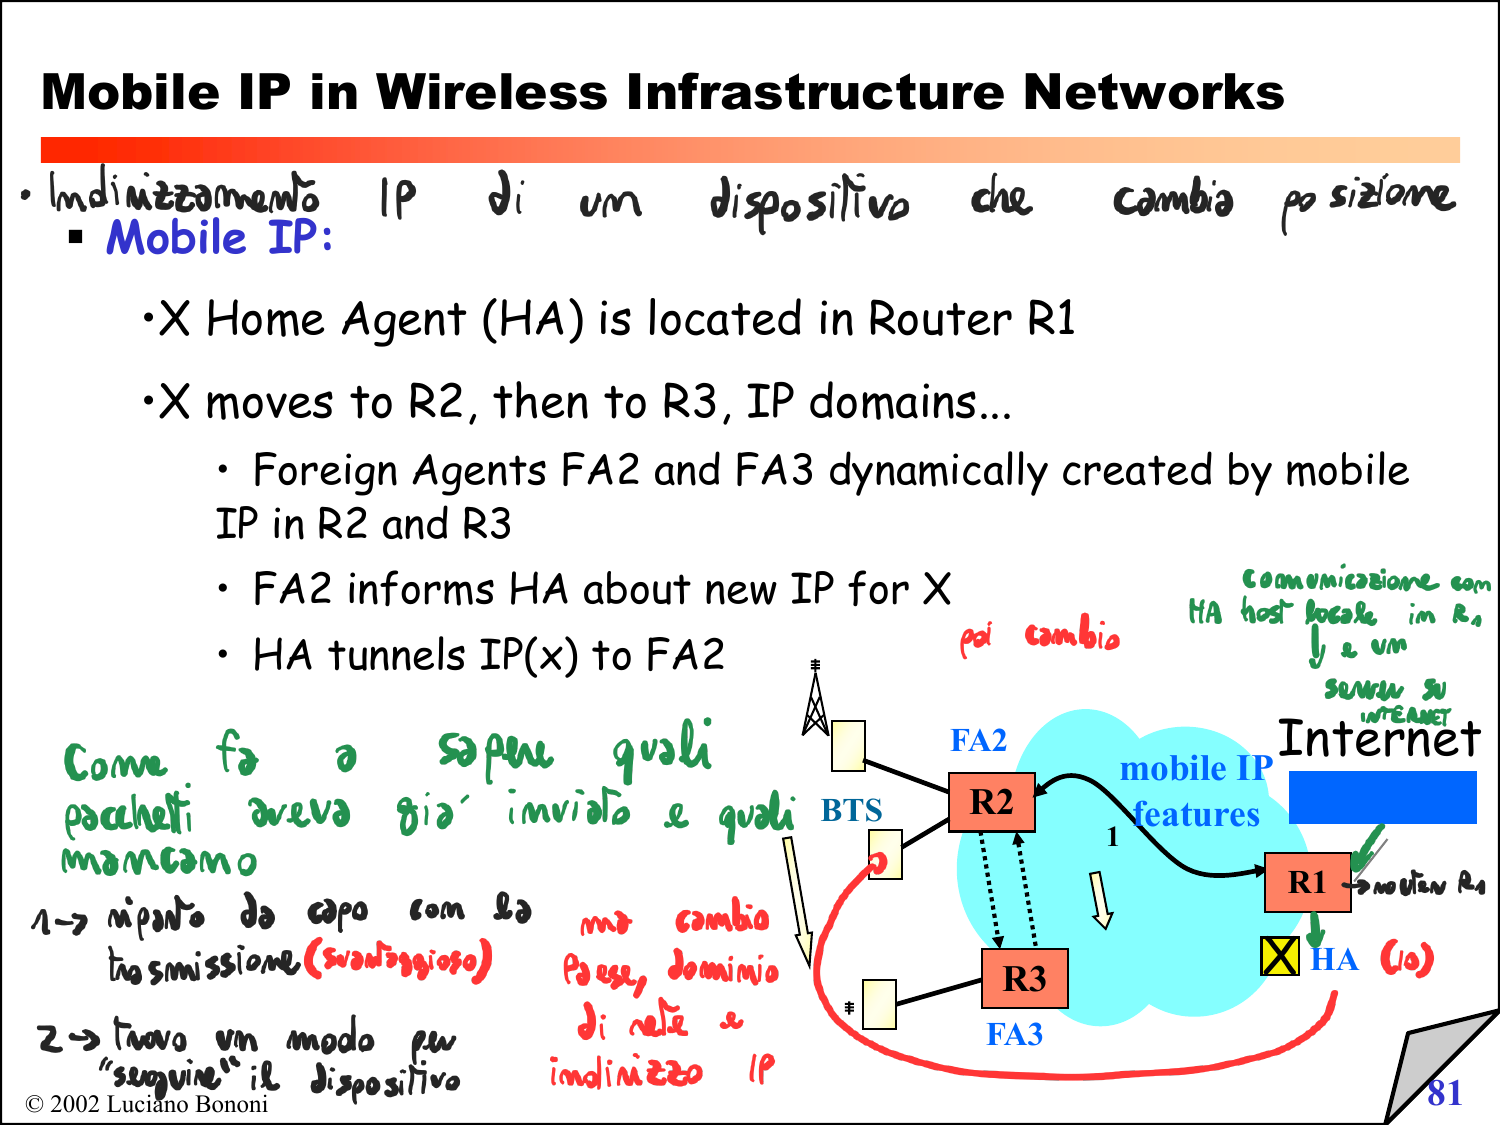
\includegraphics[width=10cm]{img/mobile_ip.png}
\end{center}

\nt{Spostamenti successivi possono creare un \emph{tunnel-in-tunnel} (FA2 che inoltra a FA3). Per evitarlo — e per evitare la \textbf{triangolazione} (tutto il traffico che passa per l'HA) — si aggiorna l'HA con il FA corrente, ottimizzando il percorso.}

\section{TCP sulle reti wireless}
TCP fornisce consegna affidabile e ordinata, con controllo di flusso e di congestione, su un IP che può perdere, duplicare e riordinare i pacchetti. Vediamo i meccanismi e poi il problema specifico del wireless.

\subsection{Da Stop \& Wait al pipelining}
Nel protocollo \textbf{Stop \& Wait} il mittente invia un segmento e attende l'ACK prima del successivo. Perdita e alterazione si gestiscono con feedback ACK/NAK, ritrasmissione, timeout e numeri di sequenza. Il problema sono le prestazioni:
$$ \text{Utilizzo del canale} = \frac{T_{tx}}{RTT + T_{tx}}, \qquad T_{tx} = \frac{\text{Size(pacchetto)}}{\text{bitrate}} $$

\ex{Inefficienza dello Stop \& Wait}{
    Segmenti da 1000 Byte, rete a 1 Gbps, $RTT = 30$ ms:
    $$ T_{tx} = \frac{8000\ \text{bit}}{2^{30}\ \text{bps}} \approx 8\ \mu s, \qquad \text{Utilizzo} = \frac{8}{8 + 30000} \approx 0{,}027\%. $$
    Su una rete da 1 Gbps si ottiene un throughput effettivo di appena $\sim$266 kbps: utilizzo bassissimo.
}

\dfn{Prodotto Banda $\times$ Ritardo}{
    Il prodotto \textbf{Bandwidth $\times$ Delay} rappresenta la quantità di dati "in transito" sulla rete (effetto memoria/pipeline). Idealmente lo si dovrebbe sfruttare interamente per massimizzare il throughput: con la pipeline piena, al destinatario arrivano dati al ritmo pieno della rete.
}

Nella \textbf{gestione a pipeline} non si attende l'ACK dei segmenti precedenti prima di inviare i successivi: aumentano i numeri di sequenza e servono buffer su mittente e destinatario. Due tecniche gestiscono errori/perdite:
\begin{itemize}
    \item \textbf{Go-Back-N (GBN)}: finestra scorrevole di $N$ segmenti in sospeso; \textbf{ACK cumulativi} ($Ack(n)$ conferma tutti i segmenti fino a $n-1$); il destinatario scarta i segmenti fuori ordine (buffer semplice, solo \texttt{Expected\_seq\#}); in caso di timeout (solo sul \texttt{send\_base}) si ritrasmettono \emph{tutti} i segmenti successivi della finestra.
    \item \textbf{Selective Repeat (SR)}: il destinatario bufferizza i segmenti fuori ordine entro la finestra di ricezione e invia ACK \emph{specifici}; il mittente gestisce un timer logico per ogni segmento in sospeso e ritrasmette solo quelli mancanti.
\end{itemize}

\nt{Perché $N$ deve essere limitato? Per il \textbf{controllo di flusso} e di \textbf{congestione}: $N = \min(\text{buffer del destinatario},\ \text{capacità del router più lento})$. Con $N$ troppo grande, un errore costringerebbe a ritrasmettere molti segmenti, saturando la rete.}

\subsection{Meccanismi di TCP}
\begin{itemize}
    \item \textbf{ACK cumulativi}: un nuovo ACK cumulativo è generato solo alla ricezione di un nuovo segmento \emph{in sequenza}.
    \item \textbf{Duplicate ACK (dupack)}: generato ogni volta che arriva un segmento \emph{fuori ordine}.
    \item \textbf{Finestra di controllo di flusso}: la dimensione della finestra è il minimo tra la \textit{advertised window} del ricevitore (spazio di buffer) e la \textbf{congestion window} (cwnd), determinata dal mittente in base al feedback della rete. La dimensione ideale è il prodotto Banda$\times$Ritardo.
    \item \textbf{Rilevazione delle perdite}: tramite \textbf{Retransmission Timeout (RTO)}, calcolato dinamicamente; oppure tramite \textbf{Fast Retransmit} — alla ricezione di \emph{tre dupack consecutivi} il mittente assume che il segmento sia perso e lo ritrasmette subito, senza attendere il timeout.
\end{itemize}

\subsection{Controllo di congestione}
\dfn{Slow Start e Congestion Avoidance}{
    In \textbf{Slow Start} la \texttt{cwnd} cresce \emph{esponenzialmente} nel tempo (raddoppia ogni RTT). Raggiunta la soglia \texttt{ssthresh}, si passa a \textbf{Congestion Avoidance}, in cui la \texttt{cwnd} cresce \emph{linearmente}. Rilevata una perdita, TCP assume congestione e riduce drasticamente la finestra.
}

\begin{center}
    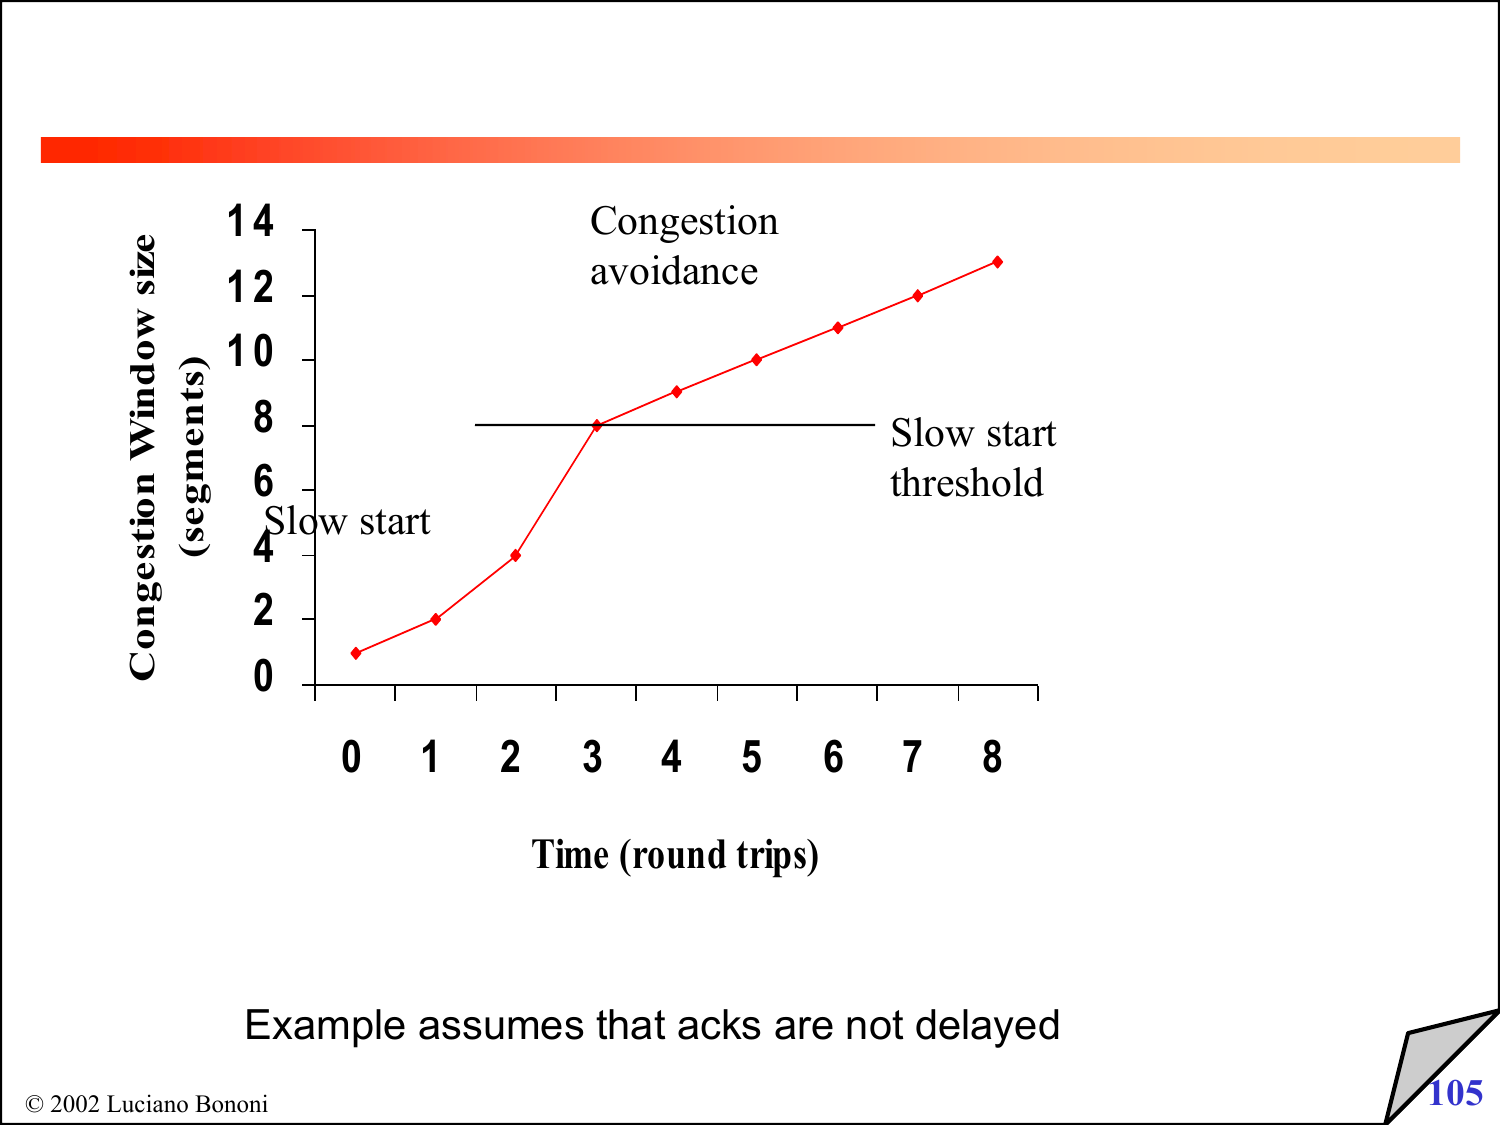
\includegraphics[width=10cm]{img/tcp_congestion_window.png}
\end{center}

\begin{itemize}
    \item Su \textbf{timeout}: \texttt{cwnd} torna al valore iniziale (1 MSS), \texttt{ssthresh} viene posta a metà della finestra precedente alla perdita, e riparte lo Slow Start.
    \item Su \textbf{fast retransmit}: la finestra viene dimezzata (fast recovery) senza ripartire da 1, perché la ricezione dei dupack indica che la rete sta ancora consegnando pacchetti.
\end{itemize}

\subsection{Il problema di TCP sul wireless}
\qs{Perché TCP soffre sulle reti wireless e multi-hop?}{
    TCP interpreta \emph{ogni} perdita come sintomo di \textbf{congestione} e reagisce riducendo la finestra. Ma nel wireless le perdite sono spesso dovute a \textbf{errori del canale} (rumore, fading) o a \textbf{rotte spezzate} dalla mobilità (es. cache DSR obsolete che fanno tentare più rotte invalide), non a congestione. La riduzione della finestra è quindi inutile e penalizza gravemente il throughput. Questo \emph{cross-layer mismatch} tra perdite da congestione e perdite da canale è il problema centrale di TCP su wireless.
}
